\begin{table}[H]
    \centering
    \begin{tabular}{lccccc}
        \hline
        \textbf{Modelo} & \textbf{Épocas} & \textbf{PSNR (dB)$\uparrow$} & \textbf{SSIM$\uparrow$} & \textbf{MAE$\downarrow$} & \textbf{SAM ($^\circ$)$\downarrow$} \\
        \hline
        DDPM condicional & 15 & 16.19 & 0.311 & 0.1293 & 49.40 \\
        DDPM condicional & 30 & 18.46 & 0.180 & 0.1046 & 48.51 \\
        DBCR-S            & 15 & \textbf{27.58} & \textbf{0.807} & \textbf{0.0313} & 12.78 \\
        DBCR-S            & 30 & 26.70 & 0.798 & 0.0339 & \textbf{11.13} \\
        \hline
    \end{tabular}
    \caption{Comparación de las métricas sobre el set de testeo de los modelos sin información SAR.}
    \label{tab:sin_sar}
\end{table}

Al analizar la tabla~\ref{tab:sin_sar} se puede concluir que el DDPM condicional clásico queda muy por debajo de DBCR-S en todas las métricas, incluso después de duplicar las épocas de entrenamiento. Más llamativo aún, su SSIM empeora al pasar de 15 a 30 épocas (0.311 a 0.180), lo que sugiere que el modelo no logra estabilizarse en ese rango de entrenamiento, probablemente porque el proceso DDPM puro parte de ruido gaussiano completo y necesita muchas más iteraciones para converger en una tarea de traducción condicional como esta. En contraste, DBCR-S alcanza un desempeño sólido ya a las 15 épocas, y extender el entrenamiento no mejora PSNR/SSIM (incluso empeora levemente), aunque sí reduce el SAM, lo que indicaría una posible saturación temprana del modelo.


\begin{table}[H]
    \centering
 
    \begin{tabular}{lccccc}
        \hline
        \textbf{Modelo} & \textbf{Épocas} & \textbf{PSNR (dB)$\uparrow$} & \textbf{SSIM$\uparrow$} & \textbf{MAE$\downarrow$} & \textbf{SAM ($^\circ$)$\downarrow$} \\
        \hline
        % DBCR-S (sin SAR)  & 15 & 27.58 & 0.807 & 0.0313 & 12.78 \\
        % DBCR-S (sin SAR)  & 30 & 26.70 & 0.798 & 0.0339 & 11.13 \\
        DBCR-SC (concat, TL)      & 15 & 26.78 & 0.792 & 0.0343 & 10.71 \\
        DBCR-SC (concat, sin TL)  & 30 & \textbf{27.82} & 0.801 & \textbf{0.0287} & \textbf{9.81}  \\
        DBCR-SC (concat, sin TL)  & 45 & 26.92 & \textbf{0.803} & 0.0327 & 12.71  \\
        DBCR-SCN (ControlNet)     & 15 & 27.28 & 0.780 & 0.0320 & 11.05 \\
        DBCR-SCN (ControlNet)     & 30 & 26.92 & 0.781 & 0.0324 & 10.94 \\
        \hline
    \end{tabular}
    \caption{Comparación de las métricas sobre el set de testeo de las estrategias de incorporación de información SAR.}
    \label{tab:sar_strategies}

\end{table}

% Al observar la tabla~\ref{tab:sar_strategies} se concluye que incorporar SAR no genera una mejora dramática en PSNR/SSIM respecto del baseline sin SAR, pero sí consistentemente reduce el SAM, lo que indica que la información SAR aporta principalmente fidelidad espectral/angular más que reducción de error pixel a pixel.

Al observar la tabla~\ref{tab:sar_strategies} se concluye que, dentro de las variantes con SAR, la concatenación directa sin transfer learning a 30 épocas es la que mejor desempeño global obtiene, superando incluso a ControlNet pese a ser una estrategia más simple. Esto podría deberse a que ControlNet, al congelar la rama principal, limita la capacidad del modelo de adaptar sus features internas a la nueva fuente de información, o a que necesitaría más épocas para aprovechar completamente la rama de control. También se observa que la versión con transfer learning (15 épocas) obtiene peor desempeño que el baseline sin SAR, lo que sugiere que la información SAR puede aportar mejoras, pero resulta más efectiva al entrenarse desde el principio.

\begin{table}[H]
    \centering
    \begin{tabular}{lcccccc}
        \hline
        \textbf{Modelo} & \textbf{Canales} &\textbf{Épocas} & \textbf{PSNR (dB)$\uparrow$} & \textbf{SSIM$\uparrow$} & \textbf{MAE$\downarrow$} & \textbf{SAM ($^\circ$)$\downarrow$} \\
        \hline
        DBCR & 6  & 15 & 26.15 & 0.786 & 0.0347 & 12.05 \\
        DBCR  & 6    & 30 & 28.12 & 0.815 & 0.0293 & 10.47 \\
        DBCR  & 6    & 45 & 28.14 & 0.830 & 0.0283 & 10.39 \\
        DBCR  & 6    & 60 & \textbf{28.45} & \textbf{0.840} & \textbf{0.0274} & 9.82 \\
        DBCR  & 6    & 75 & 28.17 & 0.837 & 0.0284 & \textbf{9.53} \\
        DBCR  & 13   & 15 & 25.62 & 0.771 & 0.0368 & 12.71 \\
        DBCR & 13 & 30 & 27.21 & 0.834 & 0.0293 & 10.89 \\
        DBCR & 13 & 45 & 25.82 & 0.775 & 0.0366 & 12.11 \\
        \hline
    \end{tabular}
    \caption{Comparación de las métricas sobre el set de testeo del modelo DBCR con 6 y 13 canales.}
    \label{tab:dbcr_bandas}
\end{table}

En la tabla~\ref{tab:dbcr_bandas} se observa que la versión de 6 canales supera a la de 13 en la mayoría de las configuraciones evaluadas, con la excepción del SSIM a 30 épocas donde obtiene un valor levemente superior (0.834 vs. 0.815). Considerando el mejor modelo de cada configuración, la versión de 6 canales domina en las cuatro métricas, lo que sustenta la hipótesis de que hay canales que no aportan o degradan la información. A su vez el desempeño con la menor cantidad de canales continúa mejorando de forma progresiva a medida que se extiende el entrenamiento (15, 30, 45 y 60 épocas), aunque con 75 épocas todas las métricas, salvo SAM, empeoran, lo que podría significar un sobreajuste al set de entrenamiento, aunque la ausencia de un conjunto de validación impide confirmarlo.

Comparando el mejor resultado de DBCR (6 canales, 60 épocas) con el mejor modelo con SAR de la tabla~\ref{tab:sar_strategies} (DBCR-SC sin TL a 30 épocas), DBCR logra superarlo en PSNR (28.45 vs.\ 27.82 dB), SSIM (0.840 vs.\ 0.801) y MAE (0.0274 vs.\ 0.0287), aunque obtiene un SAM mínimamente peor (9.82 vs.\ 9.81). Esto podría indicar que el mecanismo de fusión por atención cruzada entre las características ópticas y SAR permite una reconstrucción global de mayor calidad que la simple concatenación.


\begin{figure}[H]
    \centering
    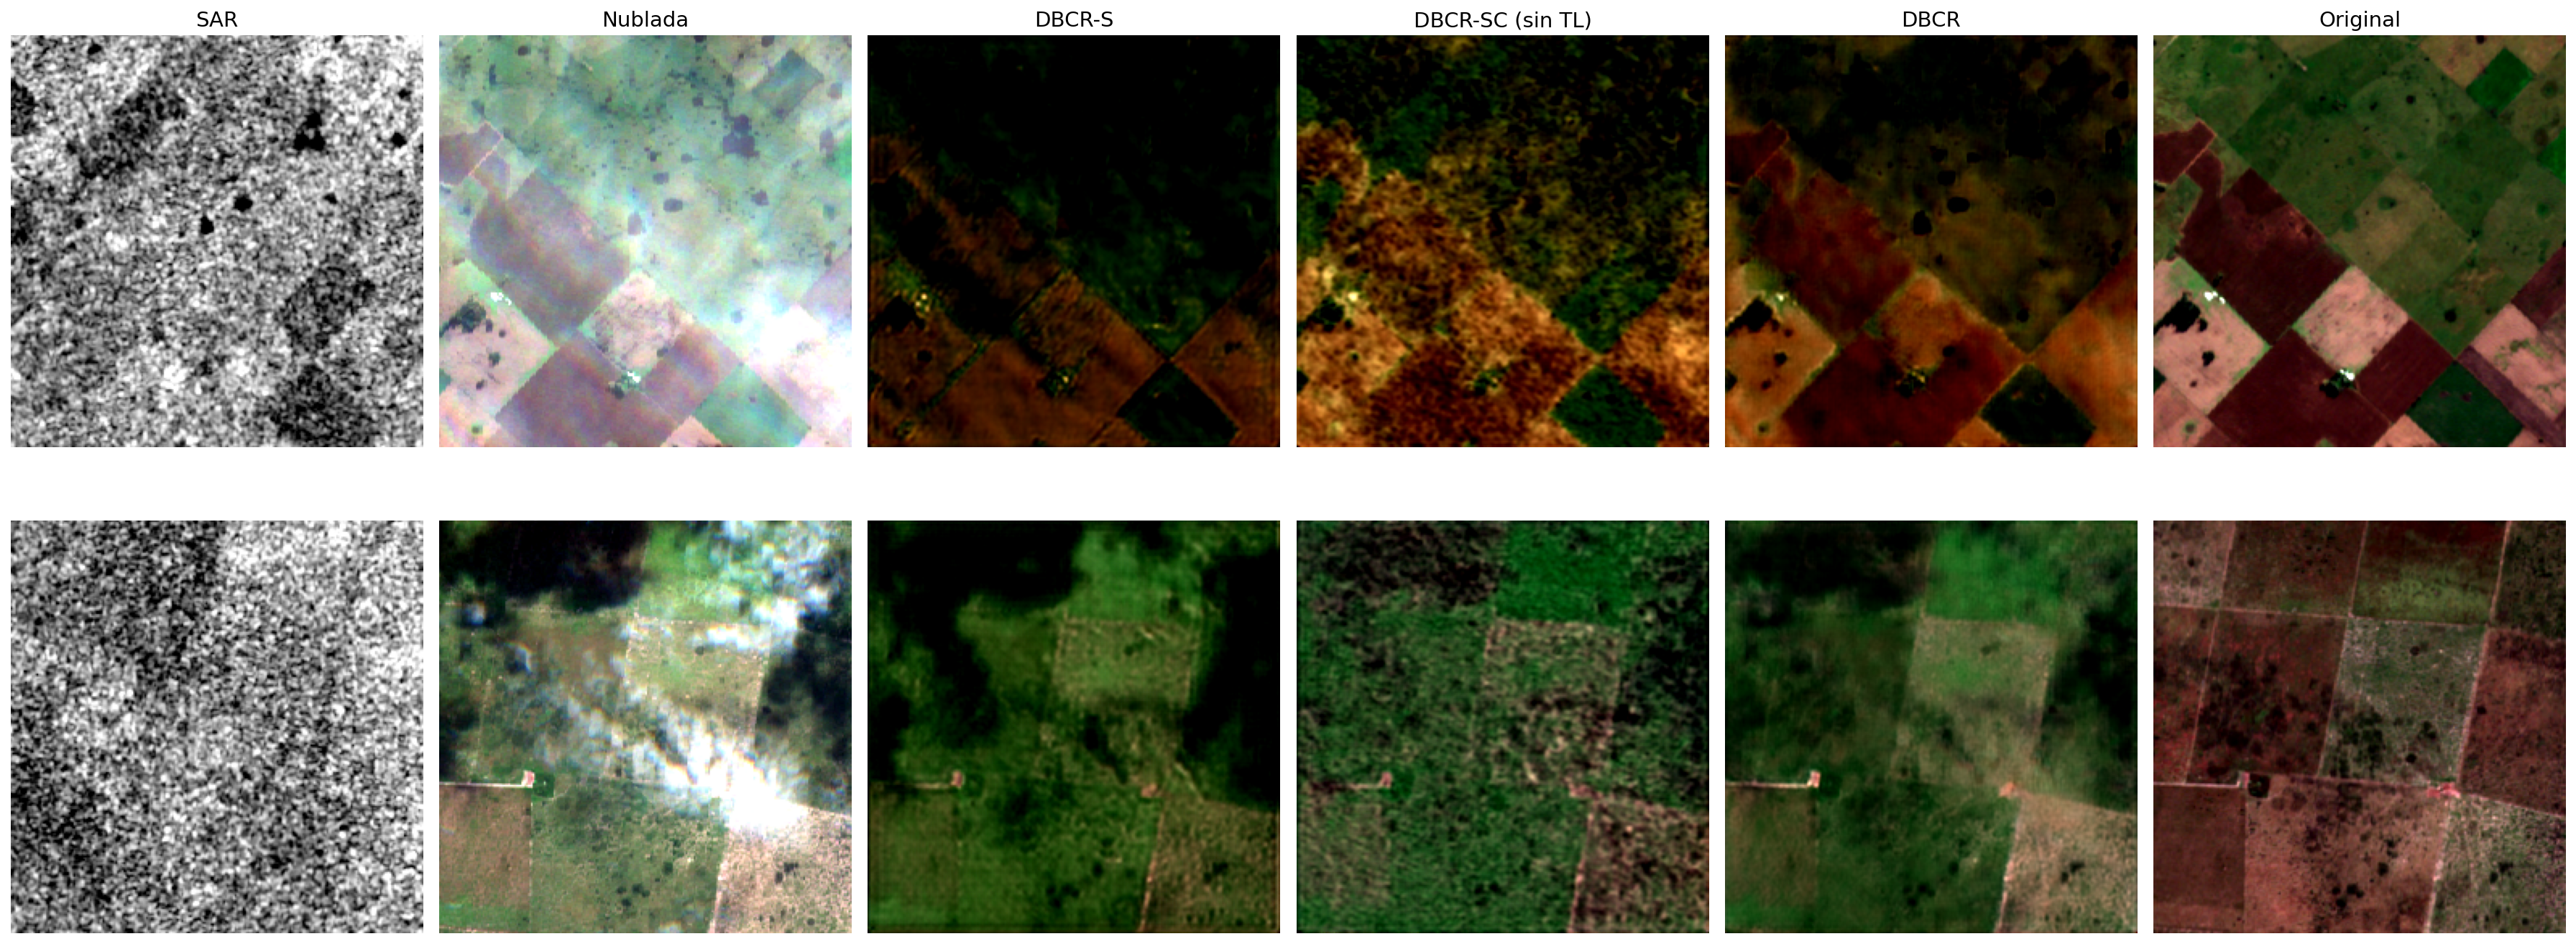
\includegraphics[width=1.0\linewidth]{../imgs/comparacion_modelos.png}
    \caption{Comparación visual sobre dos muestras del conjunto de test. De izquierda a derecha: imagen SAR, imagen nublada, reconstrucciones de DBCR-S, DBCR-SC (sin TL) y DBCR (6 bandas), e imagen de referencia.}
    \label{fig:comparacion_visual}
\end{figure}

Al observar la figura~\ref{fig:comparacion_visual} se visualiza que si bien DBCR-S logra remover las nubes de forma efectiva, tiende a mantener o generar sombras que oscurecen regiones de la imagen que en la reconstrucción original no están presentes. DBCR-SC (sin TL), por su parte, consigue eliminar la cobertura nubosa, pero introduce una textura granular y ruidosa en la reconstrucción. Este efecto es consistente con el hecho de que la concatenación directa incorpora el ruido speckle propio de la señal SAR, sin ningún mecanismo que permita al modelo separarlo, propagándolo hacia la reconstrucción final.

En contraste, DBCR presenta reconstrucciones visiblemente más suaves y sin el sombreado excesivo de DBCR-S, acercándose más a la imagen original en ambos ejemplos. Sin embargo, en la segunda fila puede verse que el modelo no logra eliminar por completo las sombras en la parte superior de la imagen, lo que indica que, si bien el mecanismo de fusión mejora sustancialmente la calidad de la reconstrucción, todavía existen casos donde persisten las sombras.

Estas observaciones sugieren que los bloques SARF permiten aprovechar la información SAR de forma más selectiva que una simple concatenación, logrando una superioridad en calidad visual, permitiendo separar entre información útil y ruido.


% \begin{figure}[H]
%     \centering
%     
\includegraphics[width=0.8\linewidth]{imgs/comparacion_steps_0.png}
%     \caption{Comparación steps}
%     \label{fig:comparacion steps}
% \end{figure}

% Con el fin de ilustrar el efecto de la cantidad de pasos de inferencia sobre la calidad de las imágenes reconstruidas, se presenta en la figura~\ref{fig:comparacion steps} una comparación visual para distintos valores de pasos, evaluada sobre DBCR. Se puede observar que con pocos pasos (e.g., 1--5) las reconstrucciones presentan artefactos y pérdida de detalle, mientras que a partir de los 10 pasos la calidad se estabiliza, con mejoras marginales al aumentar aún más la cantidad. Este comportamiento justifica la elección de 10 pasos como punto de equilibrio entre calidad de reconstrucción y eficiencia computacional.